\documentclass[10pt,a4paper]{article}
\usepackage[margin=1in]{geometry}
\usepackage[english]{babel}
\usepackage[style=apa,backend=biber]{biblatex}
\DeclareLanguageMapping{english}{english-apa}
\addbibresource{references.bib}

\usepackage{graphicx}
\usepackage{booktabs}
\usepackage{float}
\usepackage{amsmath}
\usepackage{hyperref}
\hypersetup{hidelinks}
\usepackage{tablefootnote}

\title{Economic Development and Under-5 Mortality: Analyzing Differential Returns Across Income Groups}

\author{Chen Ke Yuan Kowin (A0329512H) \protect\\
Chaisathid Patanan (A0327119E) \protect\\
Shi Boyuan (A0333653E) \protect\\
Shreya Sriram (A0327236E) \protect\\
Vivian Witjaksono (A0326440M)}


\begin{document}
		
    \maketitle 

\section{Background}

Child mortality is a key measure of development and health system effectiveness, as targeted by SDG 3.2 [\cite{un2015sdg}]. While wealthier countries generally have lower child mortality rates [\cite{swift2018}], we want to understand whether the strength of this relationship varies by development level. In low-income countries, additional income can fund basic high-impact interventions such as vaccines, clean water, and nutrition programs. In contrast, high-income countries have already addressed these preventable causes of death, so further economic growth yields smaller health gains. By testing this hypothesis in 80 countries, we seek to provide evidence on the factors that could contribute the best to achieving the SDG 3.2 targets in different development contexts.

\section{Sustainable Development Goals addressed}

\begin{itemize}
    \item SDG 3 (Good Health and Well-being)
    \item SDG 8 (Decent Work and Economic Growth)
    \item SDG 10 (Reduced Inequalities)
\end{itemize} 

\section{Objective \& Hypothesis}

\subsection{Objective}
To investigate whether income level moderates the relationship between economic development and under-5 mortality rates.

\subsection{Hypothesis Testing}
$H_{0}$: The relationship between GDP per capita and under-5 mortality is uniform across all development levels.
\\
\\$H_{a}$: Low-income countries experience significantly larger reductions in under-5 mortality per unit increase in GDP per capita compared to high-income countries ($\beta_{interaction}\neq 0$), reflecting differential returns to economic development across income levels.
    
\section{Method}
\subsection{Data \& Exploratory Data Analysis}
    \begin{tabular}{ll}
        \toprule
        \textbf{Attribute} & \textbf{Source} \\
        \midrule
        Under-5 mortality & \href{https://ourworldindata.org/grapher/child-mortality}{https://ourworldindata.org/grapher/child-mortality} \\
        GDP per capita & \href{https://data.worldbank.org/indicator/NY.GDP.PCAP.PP.KD}{https://data.worldbank.org/indicator/NY.GDP.PCAP.PP.KD} \\
        Income Classification & \href{https://ourworldindata.org/grapher/world-bank-income-groups}{https://ourworldindata.org/grapher/world-bank-income-groups} \\
        Health expenditure & \href{https://data.worldbank.org/indicator/SH.XPD.CHEX.GD.ZS}{https://data.worldbank.org/indicator/SH.XPD.CHEX.GD.ZS} \\
        DPT3 immunization & \href{https://data.worldbank.org/indicator/SH.IMM.IDPT}{https://data.worldbank.org/indicator/SH.IMM.IDPT} \\
        Population density & \href{https://data.worldbank.org/indicator/EN.POP.DNST}{https://data.worldbank.org/indicator/EN.POP.DNST} \\
        Access to safely managed drinking water & \href{https://data.worldbank.org/indicator/SH.H2O.SMDW.ZS}{https://data.worldbank.org/indicator/SH.H2O.SMDW.ZS} \\
        \bottomrule   
    \end{tabular} \\
    Under-5 mortality (SDG Indicator 3.2.1), DPT3 immunization (SDG Indicator 3.b.1), Access to safely managed drinking water (SDG Indicator 6.1.1) are classified as Tier 1 as per the Tier Classification for Global SDG Indicators, the other attributes are supporting statistics used in analysis. While GDP per capita and income classification [\cite{worldbank2024}] relate to the broader themes of SDG 8 (Economic Growth) and SDG 10 (Reduced Inequalities), they serve as contextual variables rather than official SDG indicators in our analysis.
    
    We merged and cleaned data from 2000-2021 across all countries, excluding countries with over 40\% missing attributes to balance data retention with imputation reliability, resulting in 1760 observations across 80 countries. We imputed missing values using time series methods (linear interpolation) \& central tendency measures (median/mode) and transformed inputs \& target to approximate normality \& satisfy OLS assumptions: log transformation for right-skewed variables (GDP per capita, population density, child mortality), with Box-Cox applied to the target variable [\cite{boxcox_howto}]. We then standardized all numerical variables and one-hot encoded income classification (see Appendix A for details).

    \begin{figure}[H]
    \centering
    \begin{minipage}{0.48\textwidth}
        \centering
        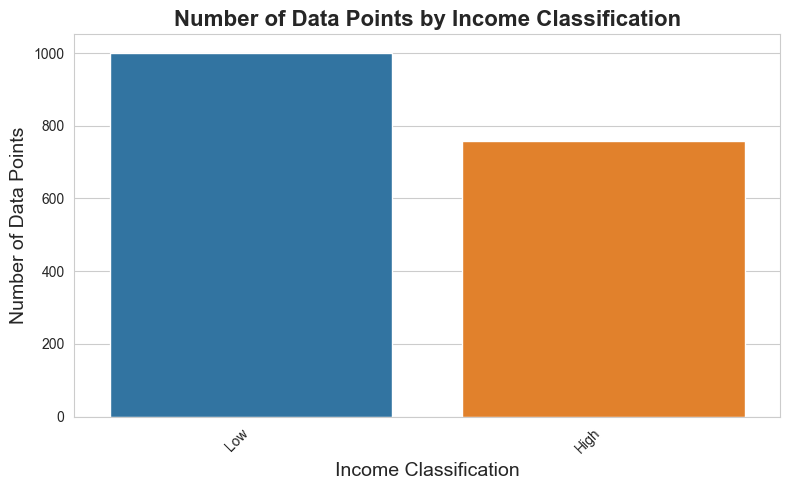
\includegraphics[width=\textwidth]{income_classification.png}
    \end{minipage}
    \hfill
    \begin{minipage}{0.48\textwidth}
        \centering
        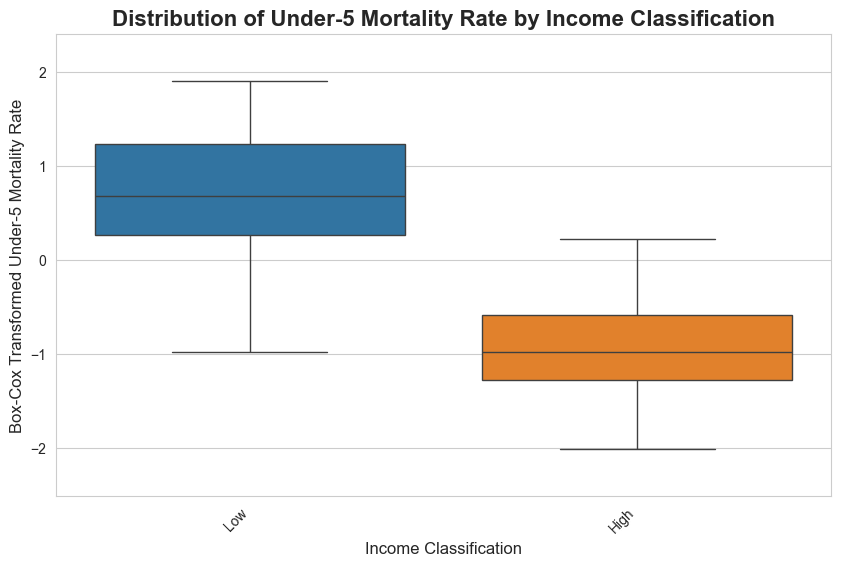
\includegraphics[width=\textwidth]{mortality_distribution_high_low.png}
    \end{minipage}
    \caption{Distribution of datapoints and mortality across income groups}
    \label{fig:both_plots}
    \end{figure}

    Figure \ref{fig:both_plots} denotes the distribution of data between the two income groups and the distribution of under-5 mortality across the income groups - the former shows we have sufficient data across the two groups, with more data for low income and the latter indicates higher mortality in the low income group compared to the high income group.

    \begin{figure}[H]
    \centering
    \begin{minipage}{0.7\textwidth}
        \centering
        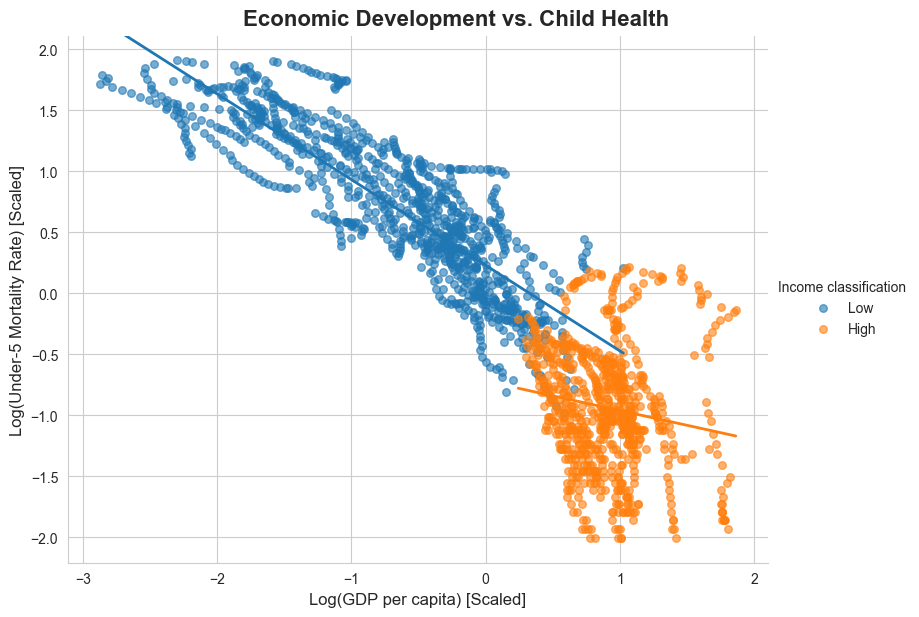
\includegraphics[width=\textwidth]{economic_development_vs_child_health.png}
    \end{minipage}
    \caption{Distribution of transformed mortality rate vs transformed GDP across income groups}
    \label{fig:mortality_gdp_transformed}
    \end{figure}

    Figure \ref{fig:mortality_gdp_transformed} reveals a steeper negative relationship between GDP and mortality in low-income countries, suggesting that economic development yields stronger mortality reductions in low-income settings compared to high-income countries where the relationship appears flatter. This visual pattern supports our hypothesis that income level moderates the GDP-mortality relationship, which we formally test using three regression approaches.

\subsection{Model specification}

We tested three modeling approaches: pooled Ordinary Least Squares, simple random effects, and Mundlak random effects (see Appendix B for pooled OLS and simple Random Effects details). \\Pooled OLS produced suggestive patterns but failed to account for country-specific heterogeneity, yielding non-significant interaction terms (p = 0.123). \\Simple random effects improved significance (p = 0.0009) by including country random intercepts [\cite{gelman2007,fitzmaurice2011}] but mixed within-country and between-country effects. \\Since our hypothesis specifically concerns between-country differences—whether low-income countries as a group experience stronger mortality reductions from GDP growth, we adopt the Random Effects with Mundlak approach [\cite{wooldridge2021}] as our primary model. This approach decomposes each time-varying predictor into its country-specific mean (capturing between-country effects) and deviations from that mean (capturing within-country effects), allowing us to isolate the between-country relationship central to our hypothesis.

As a part of Random effects with Mundlak approach [\cite{wooldridge2021}], we define country level means for \text{log\_gdp\_per\_capita}, \text{sqrt\_health\_expenditure}, \text{log\_reflected\_dpt3
\_immunization}, \text{log\_reflected\_secondary\_education},
\text{log\_population\_density}, \text{logit\_water\_services} and text{Income\_High}.

    \begin{equation}
    \begin{split}
    \text{boxcox\_mortality} \sim & 1 + \text{log\_gdp\_per\_capita} + \text{log\_gdp\_per\_capita} \times \text{Income\_High} + \\
    & \text{sqrt\_health\_expenditure} + \text{log\_reflected\_dpt3\_immunization} + \\
    & \text{log\_reflected\_secondary\_education} + \text{logit\_water\_services} + \\
    & \text{log\_population\_density} + \text{log\_gdp\_per\_capita\_mean} + \\
    & \text{log\_gdp\_per\_capita\_mean} \times \text{Income\_High\_mean} + \\
    & \text{sqrt\_health\_expenditure\_mean} + \text{log\_reflected\_dpt3\_immunization\_mean} + \\
    & \text{log\_reflected\_secondary\_education\_mean} + \text{logit\_water\_services\_mean} + \\
    & \text{log\_population\_density\_mean} + \text{TimeEffects}
    \end{split}
    \end{equation}

Model diagnostic checks including residual normality assessments are provided in Appendix C.

\section{Results}

The Random Effects model using Mundlak's approach strongly supports the hypothesis that income level moderates the GDP-mortality relationship. The between-country interaction term ($\beta = 0.9595, p = 0.0016$) demonstrates that high-income countries experience significantly weaker mortality reductions from GDP growth compared to low-income countries.

The regression results of Random Effects using Mundlak's approach are described in Figure \ref{fig:random_effects_with_mundlak}. The key coefficients from the results are described below:

\begin{itemize}
    \item \textbf{Between-country effect (Primary evidence for $H_{a}$)}:
    \\
    The coefficient of \text{log\_gdp\_per\_capita\_mean}:\text{Income\_High\_mean} is 0.9595 with the p value being 0.0016 i.e., the result is statistically significant at the 0.05 level.
    \\
    This coefficient shows that countries persistently classified as high-income experience a significantly weaker relationship between GDP per capita and under-5 mortality compared to low-income countries. The positive coefficient indicates that each unit increase in average GDP per capita is associated with smaller mortality reductions in high-income countries. This directly supports our hypothesis that low-income countries experience stronger health returns from economic growth compared to high-income countries.
    
    \item \textbf{Within-country effect (evidence for policy changes)}:
    \\ The coefficient of \text{log\_gdp\_per\_capita:Income\_High} is -0.5486 with the p value being 0.0121 i.e., the result is statistically significant at the 0.05 level.
    \\
    Within countries over time, high-income countries show a statistically different (slightly stronger) absolute response to GDP growth compared to low-income countries. This reflects that low-income countries operate in a different context—they start with higher baseline mortality, so the same absolute reduction represents a larger proportional improvement in child health outcomes.
    \end{itemize}
    
    \begin{figure}[H]
    \centering
    \begin{minipage}{0.7\textwidth}
        \centering
        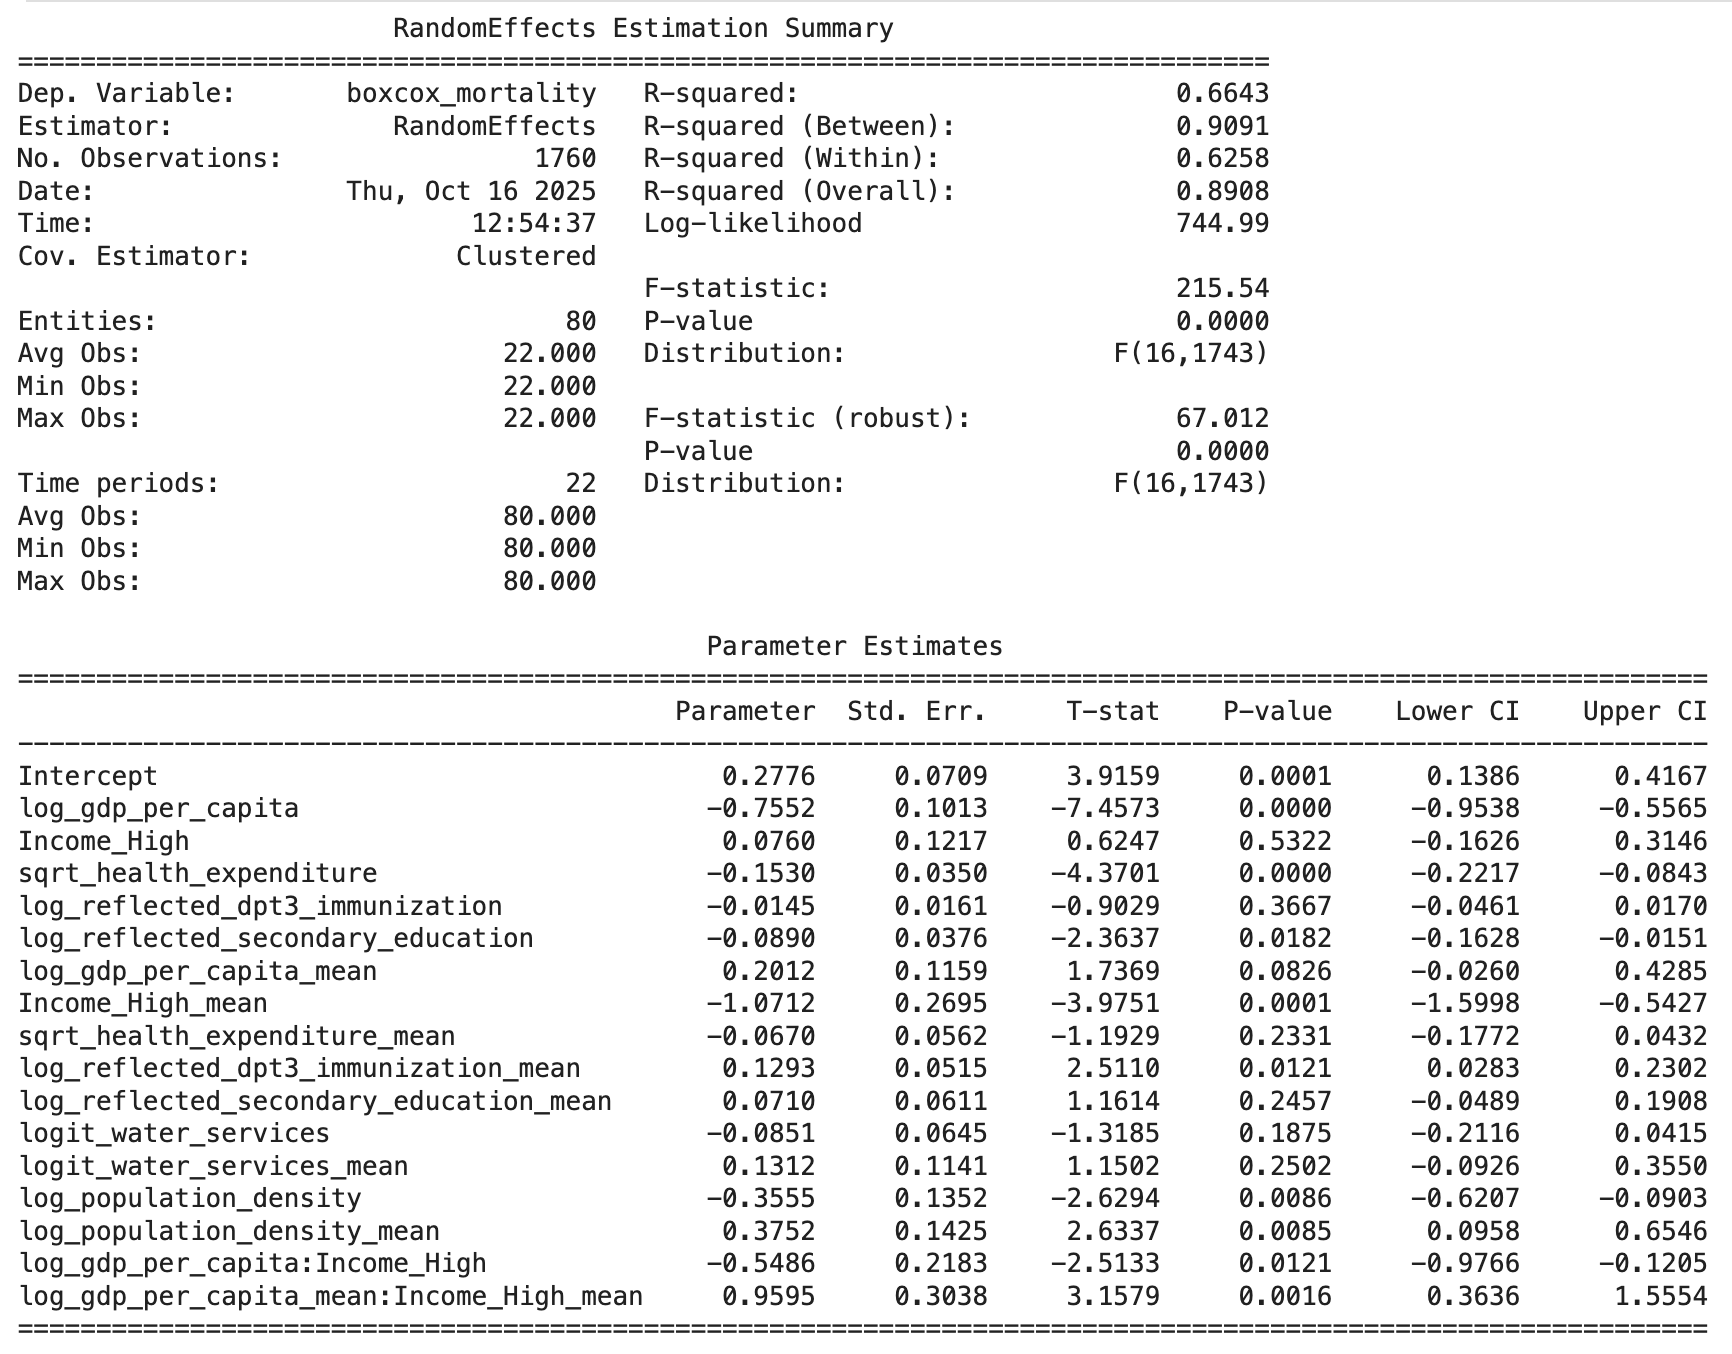
\includegraphics[width=\textwidth]{random_effects_with_mundlak_results.png}
    \end{minipage}
    \caption{Regression results of Random Effects with Mundlak approach}
    \label{fig:random_effects_with_mundlak}
    \end{figure}

    Since we scaled and normalized attributes in the preprocessing step, we scale them back so as to interpret the results in the original scale.

\section{Discussion and Conclusion}

For the purpose of interpretation, we simulate a 10\% increase in GDP across income groups, while keeping all other model inputs constant at their empirically observed or derived values from the dataset :

    \begin{figure}[H]
    \centering
    \begin{minipage}{0.7\textwidth}
        \centering
        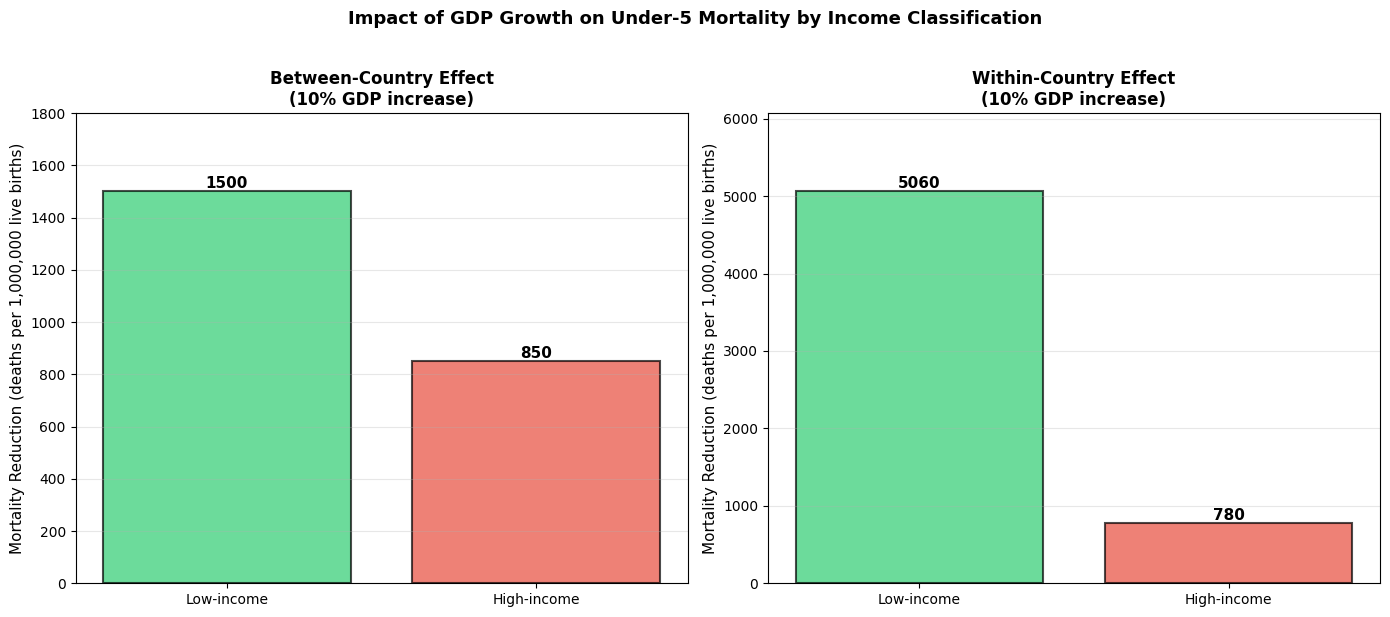
\includegraphics[width=\textwidth]{results.png}
    \end{minipage}
    \caption{Results of simulating 10\% GDP on between-country and within-country effects}
    \label{fig:simulation}
    \end{figure}

Figure \ref{fig:simulation} suggests that between countries, a 10\% GDP increase is associated with 1.76x greater mortality reduction in persistently low-income countries compared to high-income countries. Within countries, the absolute mortality reduction is larger for low-income countries (5,060 deaths averted per 1MM births) than high-income countries (780 deaths averted per 1MM births), reflecting both steeper GDP-mortality gradients and higher baseline mortality in low-income settings.

This confirms our hypothesis: low-income countries experience substantially stronger health returns from economic growth than high-income countries, supporting targeted resource allocation toward lower-income contexts to achieve SDG 3.2 targets. See Appendix D for detailed interpretation of coefficient differences.

\subsection{Future Work}
\begin{itemize}
\item \textbf{Lagged effects of predictors}: Our analysis assumes immediate effects of economic and health variables on mortality. However, improvements in GDP, health expenditure, or education may take several years to translate into mortality reductions. Future research could incorporate time lags to capture delayed impacts and identify optimal policy horizons.

\item \textbf{Income group transitions}: 14 of the 80 countries transitioned between income classifications during 2000-2021, these have been denoted as `Low and High' in Figure \ref{fig:income_classification}. While we retained them in our analysis, examining these transitioning countries separately could reveal whether the GDP-mortality relationship shifts gradually as countries develop or exhibits threshold effects at classification boundaries.

    \begin{figure}[H]
    	\centering
    	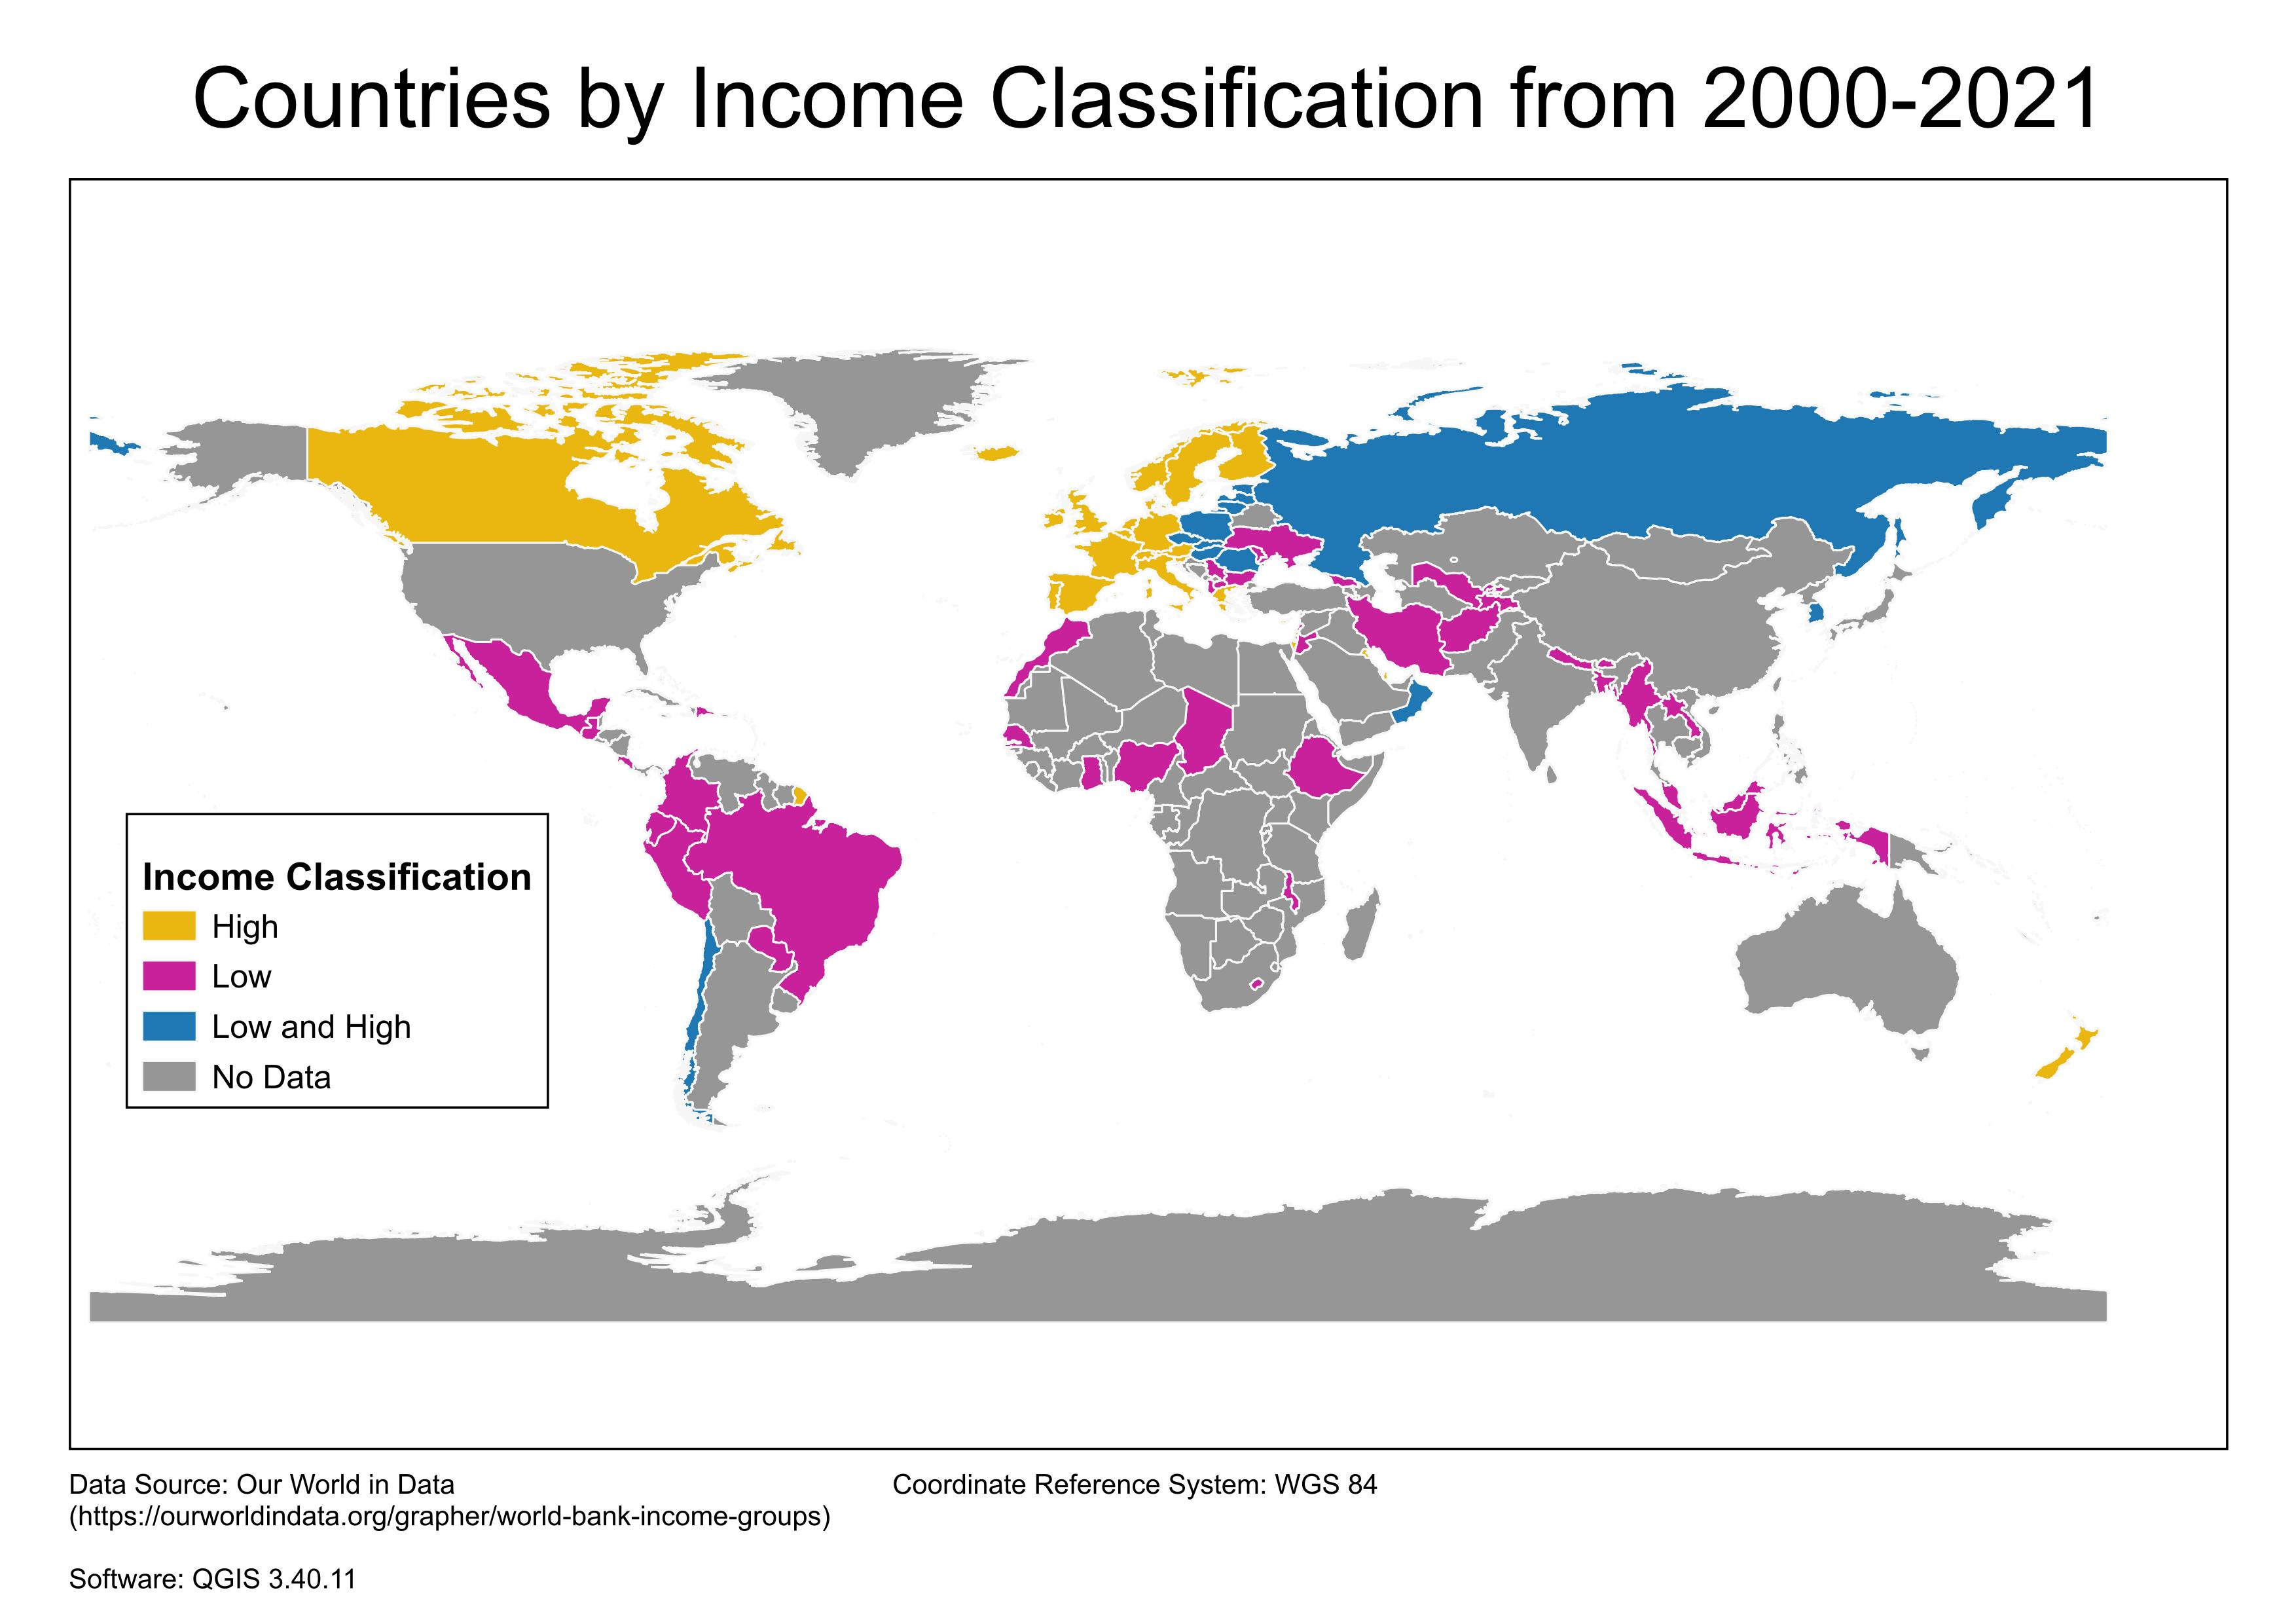
\includegraphics[width=0.7\columnwidth]{Countries by Income Classification.jpg}
    	\caption{Income classification of countries from 2000 to 2021}
    	\label{fig:income_classification}
    \end{figure}

\item \textbf{Additional mediating factors}: Incorporating variables such as governance quality, disease burden, healthcare infrastructure, and income inequality could help identify the mechanisms through which GDP affects mortality and reveal which interventions yield the highest returns in different development contexts.
\end{itemize}

\newpage
\section{References}
\printbibliography[heading=none]
	
\newpage
\section{Appendix}
\appendix
    \section{Preprocessing of Data: Cleaning, Imputation, and Scaling }
    \subsection{Data Cleaning}
    We merged the data from the different sources after ensuring a consistent format and including data from 2000 to 2021 (both years inclusive). We standardized the country names across datasets and dropped data of countries that had more than 40\% of attributes missing. The 40\% threshold ensures that the majority of each country's data comes from observed rather than imputed values, maintaining data integrity while maximizing sample size. This resulted in a dataset with 1760 rows across 80 countries.

    \subsection{Imputation}
    While processing our data, we observed missing data:    		
        \begin{table}[H]
            \centering
            \caption{Iteration 1: Missing Data statistics across attributes}
            \label{tab:table}
            \begin{tabular}{ll}
                \toprule
                \textbf{Attribute} & \textbf{Missing \%} \\
                \midrule
                Secondary education, pupils female &  22.3864 \\
                People using safely managed drinking water services & 0.6250 \\
                Population density (people per sq. km of land area) & 0.3409 \\
                Income classification & 0.3409 \\
                Current health expenditure & 0.1136 \\
                \bottomrule   
            \end{tabular} \\
            \footnotesize{Note: Attributes not noted above do not have any missing data.}\\
        \end{table}

    As the missing percentages are reasonable, we proceeded to impute the data using the following techniques:
    \begin{itemize}
    \item As educational enrollment changes gradually and predictably over time within countries, so does population density. Hence, we impute the missing values for \textit{Secondary education, pupils female} and \textit{Population density (people per sq. km of land area)} using \textbf{linear interpolation} with the country.
    \item As health expenditure and water access percentages fluctuate without predictable directional change year-to-year, we impute the missing values for \textit{Current health expenditure} and \textit{People using safely managed drinking water services} the country's \textbf{median} a more stable estimate than assuming linear progression between sparse observations.
    \item As income classifications are categorical and change infrequently—the World Bank reclassifies countries only when they cross thresholds, we impute the \textit{Income classification} using the mode within the country.
    \end{itemize}

    After this exercise, when we rechecked the missing data statistics, we see the following:

            \begin{table}[H]
            \centering
            \caption{Iteration 2: Missing Data statistics across attributes}
            \label{tab:table}
            \begin{tabular}{ll}
                \toprule
                \textbf{Attribute} & \textbf{Missing \%} \\
                \midrule
                Secondary education, pupils female &  0.7386 \\
                Population density (people per sq. km of land area) & 0.3409 \\
                \bottomrule   
            \end{tabular} \\
            \footnotesize{Note: Attributes not noted above do not have any missing data.}\\
        \end{table}

    \begin{itemize}
    \item After linear interpolation, there are remaining gaps are at series endpoints for \textit{secondary education, pupils female}, where interpolation did not work. We choose to \textbf{carry forward/backward the nearest observed value} within a country for imputation since we do not anticipate dramatic jumps between consecutive years within a country.
    \item As population density changes predictably within countries, we use the \textbf{mean} for imputation, as it provides a reasonable country-specific estimate when no temporal neighbors exist for interpolation, capturing the country's typical density level across the observed period.
    \end{itemize}

    With this second iteration, all missing data was successfully imputed.

    \subsection{Normalization, Scaling and One Hot Encoding}

    We checked the distribution of each of the attributes, the representation is in Figure \ref{fig:distribution}.
    \begin{figure}[H]
    	\centering
    	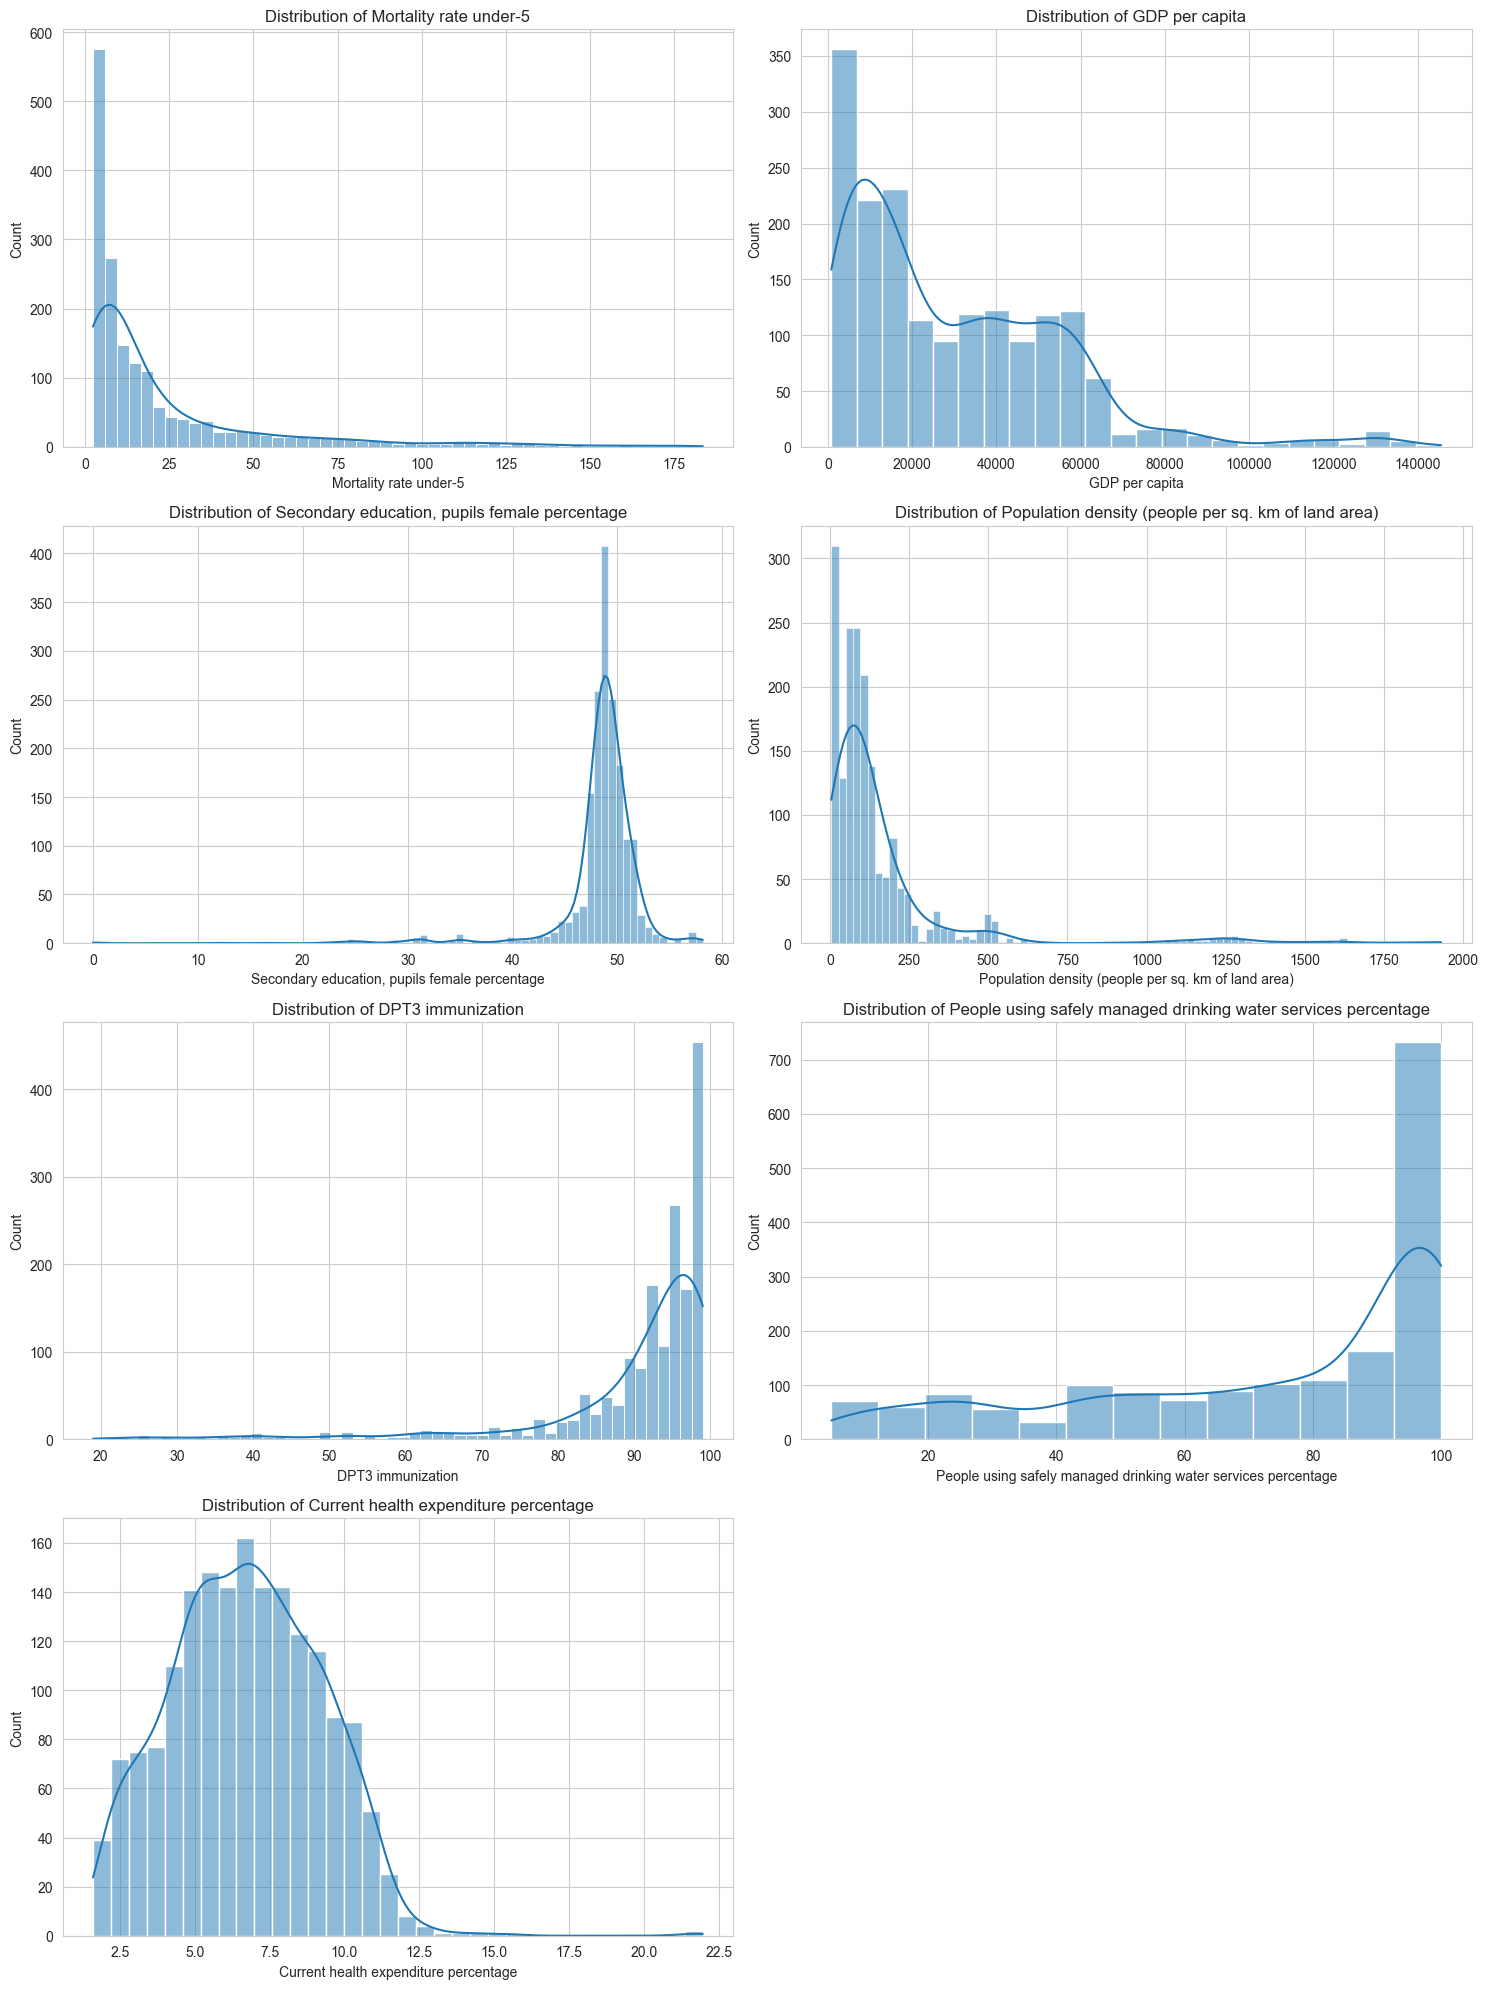
\includegraphics[width=0.7\columnwidth]{distribution_plots1.png}
    	\caption{Distribution of the inputs and the target}
    	\label{fig:distribution}
    \end{figure}

As indicated in the plots above, the following attributes are extremely right-skewed:
    \begin{itemize}
        \item GDP per capita
        \item Population density
        \item Child mortality rate
    \end{itemize}

Using log transformation for these aforementioned attributes using $np.log1p$ because many density values are close to zero, $log(0)$ is undefined. \textit{Current health expenditure percentage} has a mild positive right-skew, square root transformation is often ideal for mild positive skew as it is gentler than the log and can stabilize variance. \textit{People using safely managed drinking water services percentage} is bimodal, a logit transformation would be appropriate to use. \textit{Secondary education, pupils female percentage} is heavily left-skewed, but it has a bell shaped curve, so we leverage the reflect-and-transform technique: recentering it and doing a log transformation. Similarly, as \textit{DPT3 immunization percentage} is also left-skewed, we use reflect-and-transform technique.

    \begin{figure}[H]
    	\centering
    	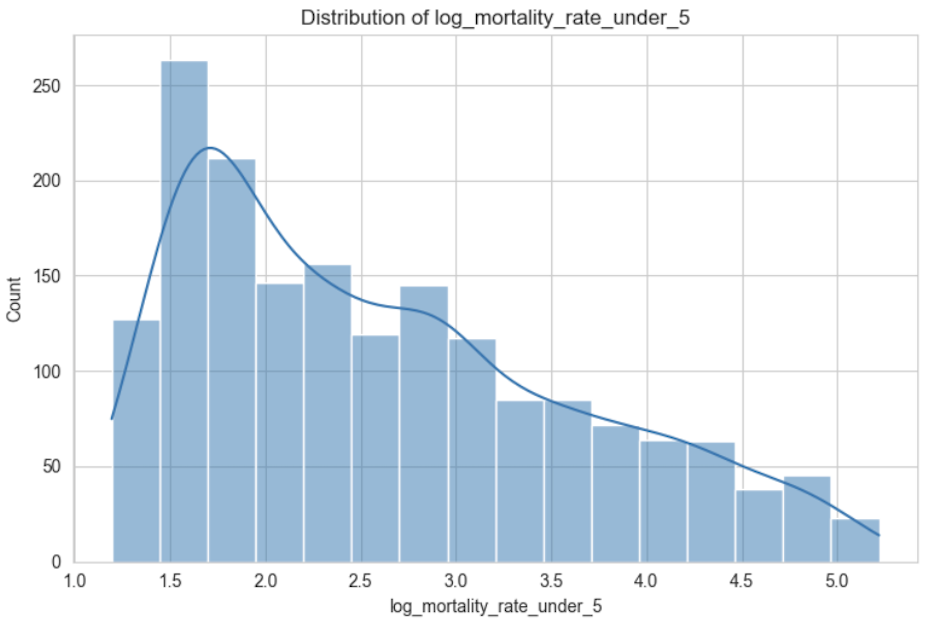
\includegraphics[width=0.35\columnwidth ]{mortality_transformation1.png}
    	\caption{Distribution of log transformed target}
    	\label{fig:distribution_after_transformed_mortality}
    \end{figure}

Since child mortality rate was still right-skewed after this exercise, as indicated in Figure \ref{fig:distribution_after_transformed_mortality}, we used Box-Cox transformation on the transformed target to make its distribution normal.

    \begin{figure}[H]
    	\centering
    	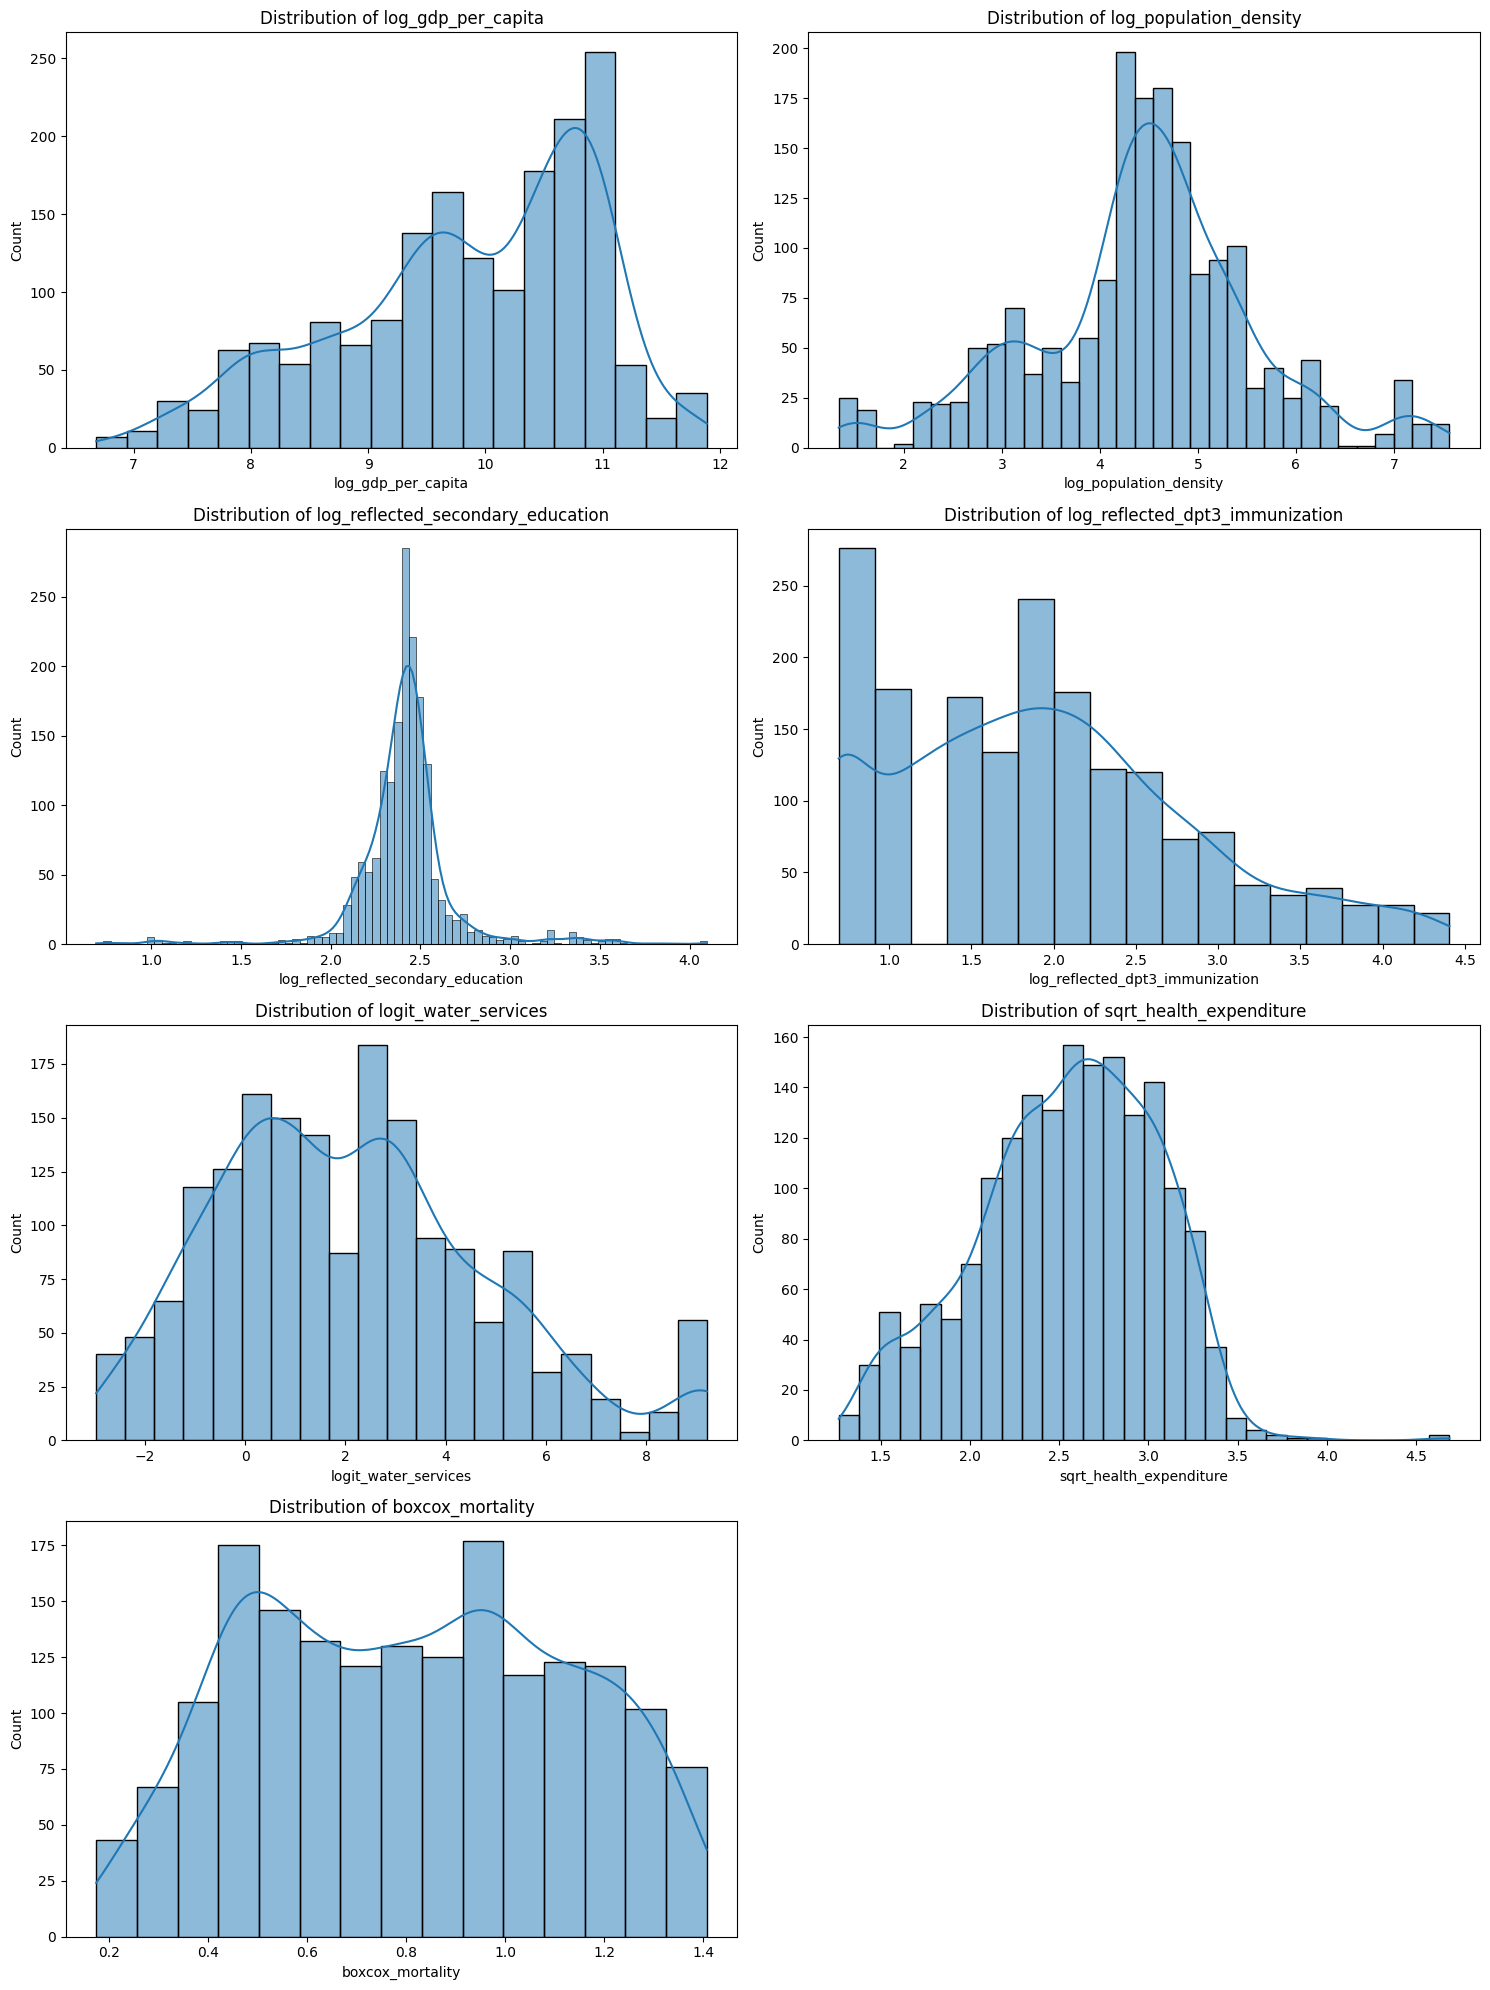
\includegraphics[width=0.7\columnwidth]{transformation_final.png}
    	\caption{Distribution of all transformed inputs and target}
    	\label{fig:post_transformation}
    \end{figure}

Post the Box-Cox transformation, all attributes are nearly normal as indicative of Figure \ref{fig:post_transformation}.
Normalizing both inputs and target variables stabilizes variance, reduces outlier influence, and helps satisfy OLS assumptions, particularly normality of residuals. This which is essential for valid hypothesis testing and reliable inference about the moderating effect of income level on the GDP-mortality relationship.

We then scale all the numerical columns using standard scaling—centering by the mean and scaling by the standard deviation.
We perform one-hot encoding for the categorical variable, income classification, so the data is ready to be used for modeling.

\section{Model Specification}

\subsection{Pooled Ordinary Least Squares}
   To test the interactions between our target and the attributes in our panel data, we start off with a simple model, Pooled Ordinary Least Squares (Pooled OLS) with standard errors clustered at the country level to account for within-country correlation over time. Representation of the model is as below :

    \begin{equation}
    \begin{split}
    \text{boxcox\_mortality} \sim & \text{log\_gdp\_per\_capita} \times \text{Income\_High} + \\
    & \text{sqrt\_health\_expenditure} + \\
    & \text{log\_reflected\_dpt3\_immunization} + \\
    & \text{log\_reflected\_secondary\_education} + \\
    & \text{logit\_water\_services} + \\
    & \text{log\_population\_density} + \\
    \end{split}
    \end{equation}

    \begin{figure}[H]
    \centering
    \begin{minipage}{0.7\textwidth}
        \centering
        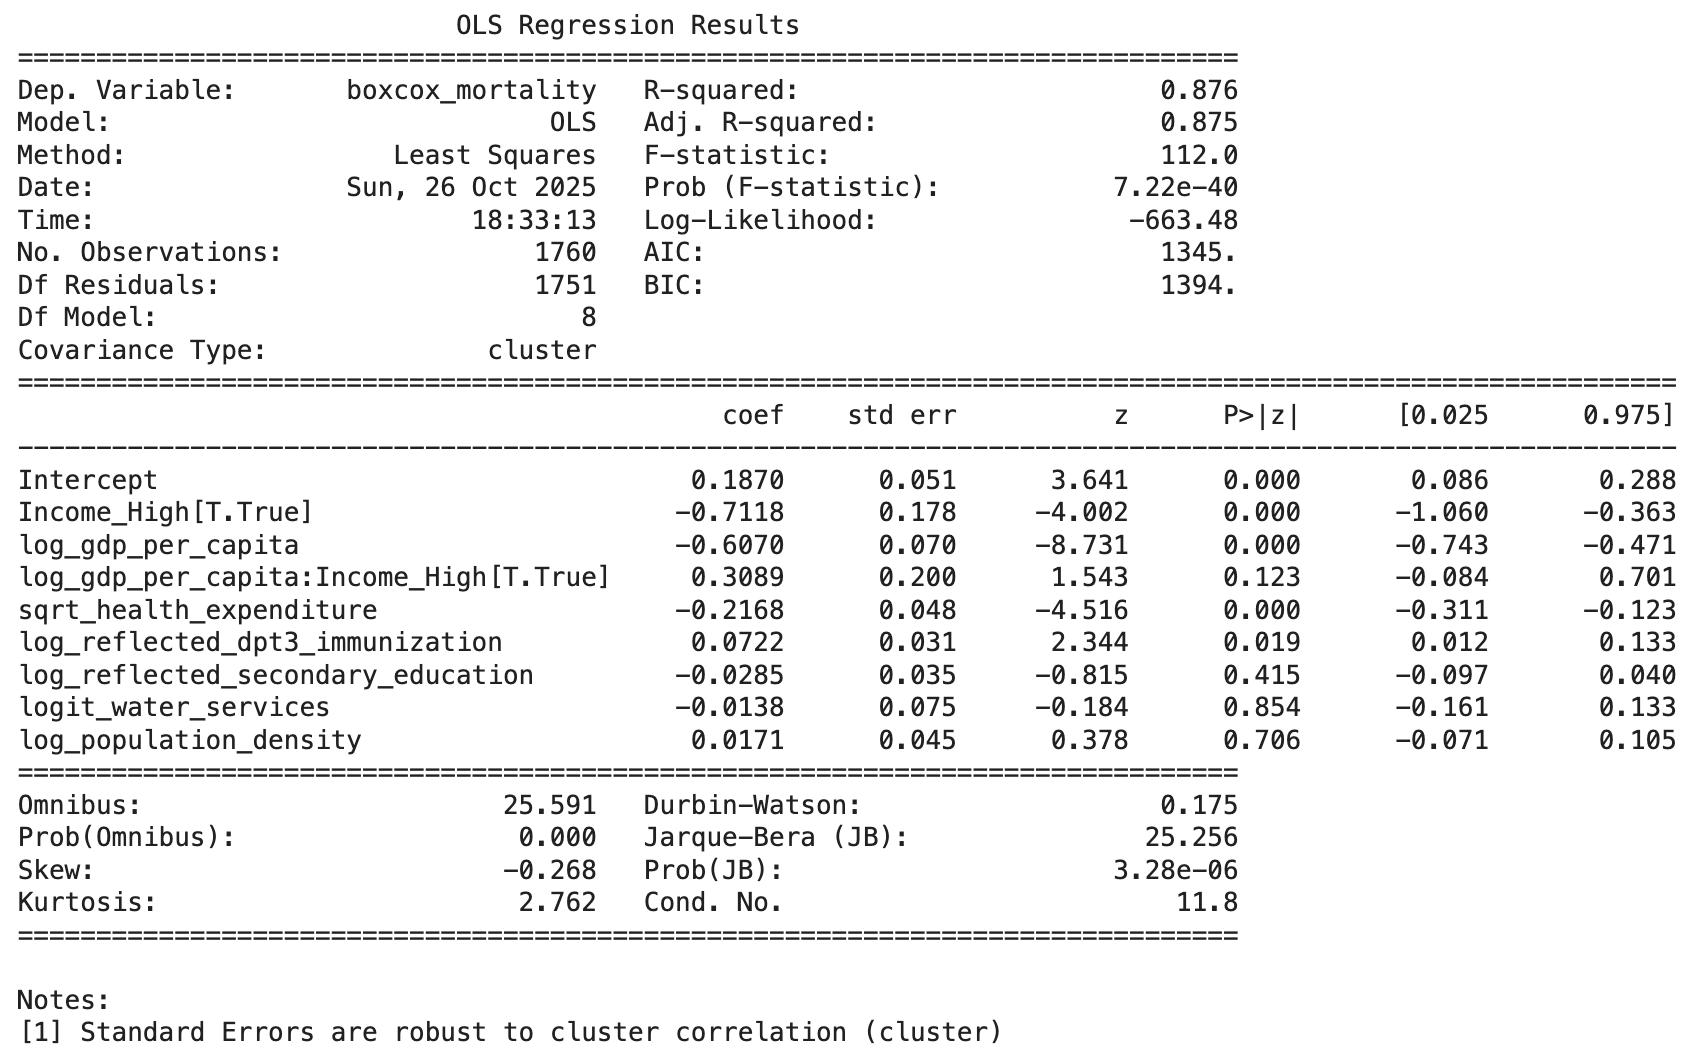
\includegraphics[width=\textwidth]{OLS_results.png}
    \end{minipage}
    \caption{Regression results for Pooled OLS}
    \label{fig:ols_regression}
    \end{figure}
    
    \begin{figure}[H]
    \centering
    \begin{minipage}{0.7\textwidth}
        \centering
        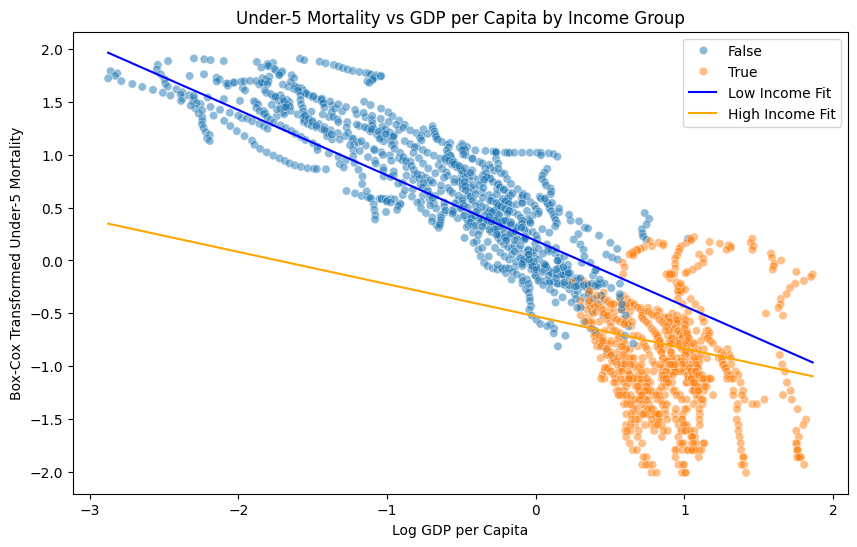
\includegraphics[width=\textwidth]{pooled_ols.png}
    \end{minipage}
    \caption{Fit for Pooled OLS}
    \label{fig:ols_fit_plot}
    \end{figure}  

    Figure \ref{fig:ols_fit_plot} indicates steeper negative slopes for the low-income group as compared to high-income group, as also noted in Figure 2. 
    
   Pooled OLS produces suggestive results: Low-income countries show a steeper GDP-mortality gradient (0.62 units) compared to high-income countries (0.31 units); the model fit has a high $R^{2}$ of 0.875 yet the difference between the GDP-mortality gradients for the income groups is not statistically significant at the 0.05 level (p-value = 0.123) as indicated in Figure \ref{fig:ols_regression}.
   
   A fundamental limitation of pooled OLS is that it assumes that countries are homogeneous except for measured predictors. In practice, countries differ substantially in unmeasured dimensions—institutional quality, geographic characteristics, and healthcare system maturity—that independently affect child mortality. When these country-specific factors are omitted, they remain in the error term, introducing bias and inflating standard errors that mask genuine patterns.
   
   To address this, we employ a random effects model, which allows each country to have a country-specific baseline while maintaining a common relationship between GDP and mortality.

   \subsection{Random effects model}
   Random Effects Model assumes that individual country effects are uncorrelated with the explanatory variables [\cite{gelman2007,fitzmaurice2011}]. This allows for the inclusion of time-invariant variables, which is not possible in fixed effects models. The country-specific random intercept captures unmeasured time-invariant characteristics (such as geography or cultural factors) that affect baseline mortality levels.

    \begin{equation}
    \begin{split}
    \text{boxcox\_mortality} \sim & 1 + \text{log\_gdp\_per\_capita} + \\
    & \text{log\_gdp\_per\_capita} \times \text{Income\_High} + \\
    & \text{sqrt\_health\_expenditure} + \\
    & \text{log\_reflected\_dpt3\_immunization} + \\
    & \text{log\_reflected\_secondary\_education} + \\
    & \text{logit\_water\_services} + \\
    & \text{log\_population\_density} + \\
    & \text{TimeEffects}
    \end{split}
    \end{equation}

    \begin{figure}[H]
    \centering
    \begin{minipage}{0.7\textwidth}
        \centering
        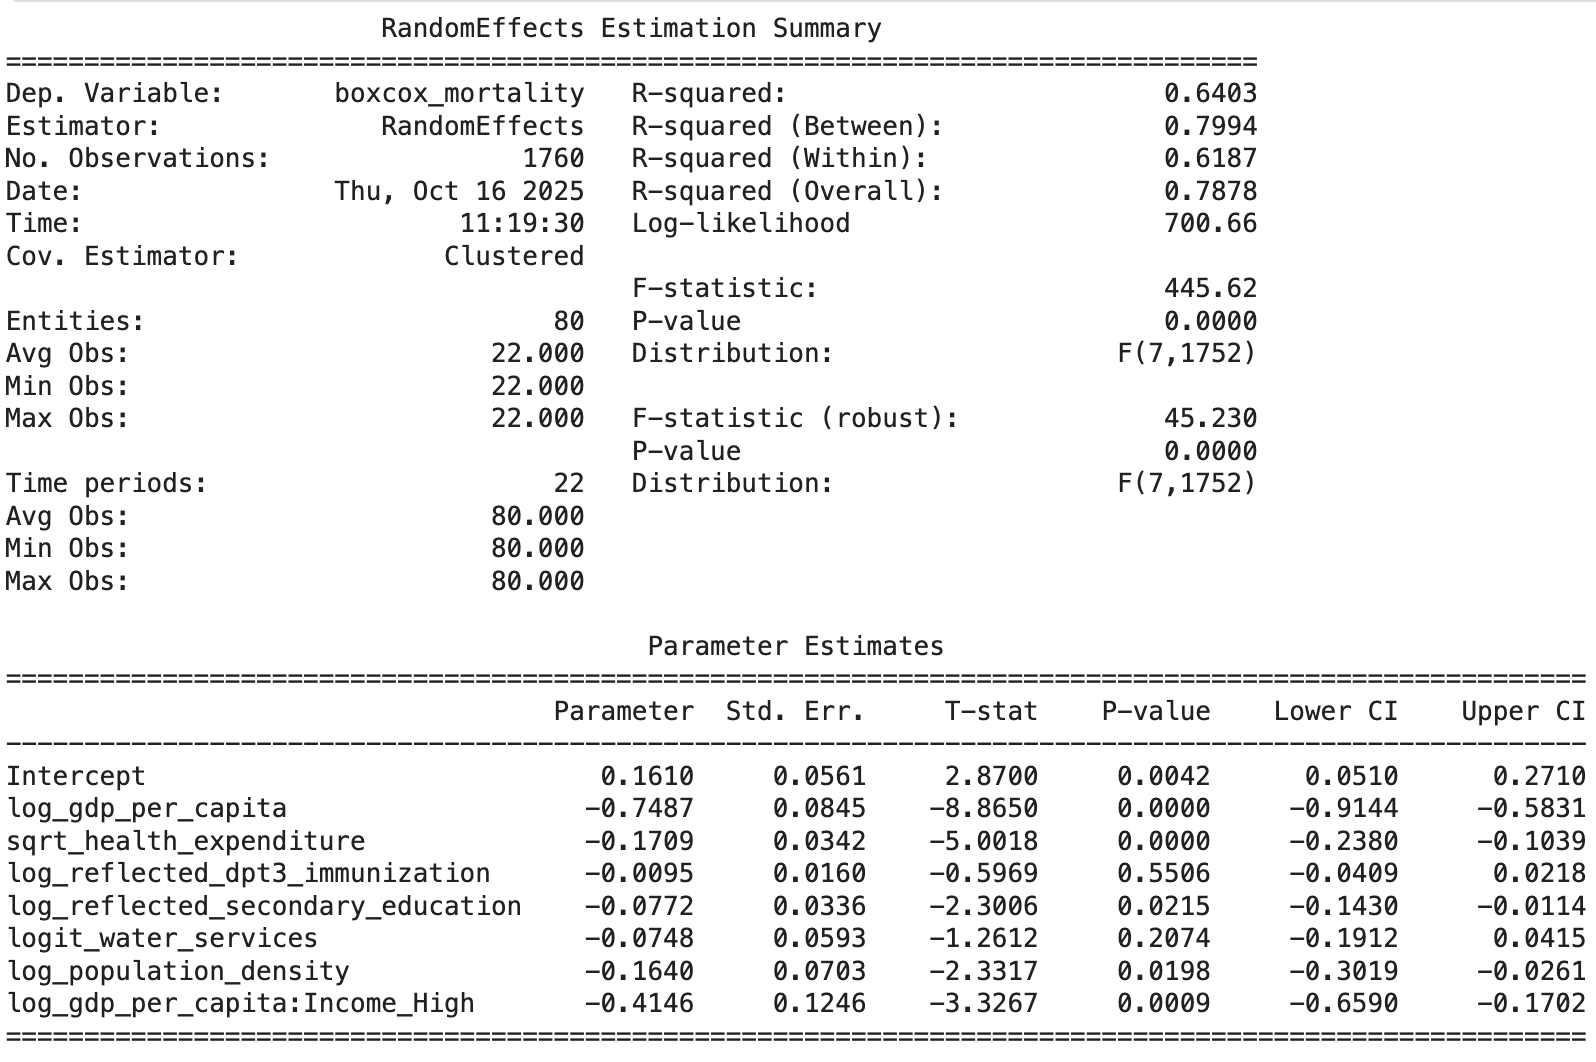
\includegraphics[width=\textwidth]{random_effects_results.png}
    \end{minipage}
    \caption{Regression results for simple Random Effects}
    \label{fig:random_effects_regression}
    \end{figure}    

    The random effects model permits each country to have a country -specific baseline while maintaining a common relationship between GDP and mortality. By explicitly controlling for time-invariant country heterogeneity, the model isolates the effect of measured variables. This approach successfully reveals the underlying pattern: the GDP × Income interaction term becomes statistically significant at the 0.05 level (p = 0.0009) as indicated in Figure \ref{fig:random_effects_regression}, indicating that accounting for country-level differences uncovers the genuine relationship obscured by pooled OLS.
    
    While the random effects model improves our results significantly, a key limitation remains: it assumes that unmeasured country characteristics (such as institutional quality or healthcare system development) are unrelated to GDP, which is unrealistic. In reality, countries with well-developed institutions (educational, health, governmental) tend to have both higher GDP and better health outcomes. Ignoring these factors potentially introduces bias in our estimates.
    
    Simple random effects mixes the within-country and between-country effects of how GDP affects child mortality. Our hypothesis about diminishing returns in low-income countries specifically concerns the between-country aspect—that low-income countries as a group experience stronger mortality reductions from economic growth compared to high-income countries. So it is valuable to split the two effects using Mundlak's approach to isolate the between-country relationship that our hypothesis addresses.

\section{Random Effects Model using Mundlak Approach: Diagnostics}
We assessed normality assumptions for our Random Effects Mundlak model at two levels: within-country residuals and between-country residuals.

Figure X shows Q-Q plots and histograms for both components. Both plots follow reasonable normality with only minor tail deviations, these diagnostics support the validity of our model-based inference.

    \begin{figure}[H]
    \centering
    \begin{minipage}{0.7\textwidth}
        \centering
        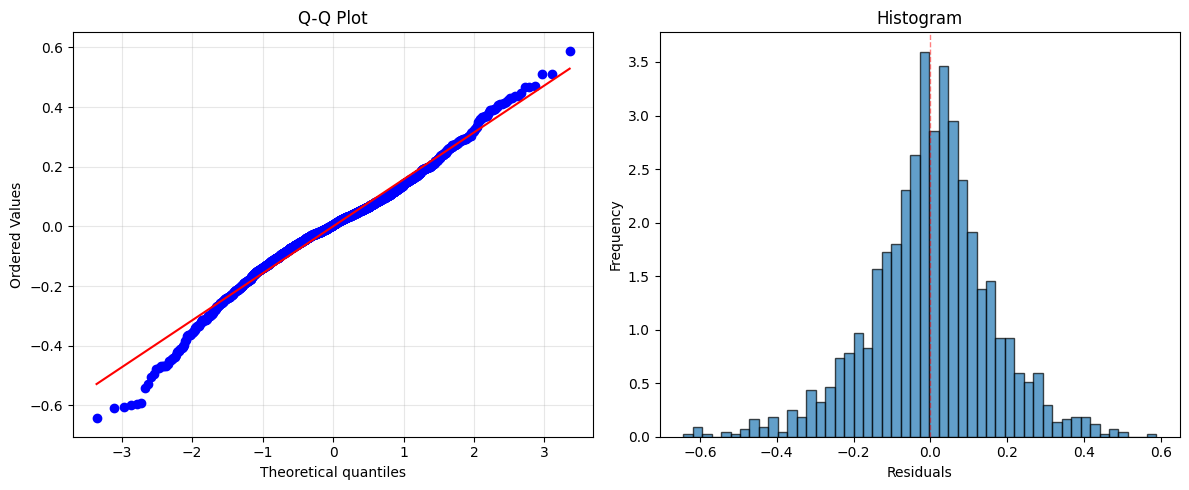
\includegraphics[width=\textwidth]{qq1.png}
    \end{minipage}
    \caption{Within-country residuals}
    \begin{minipage}{0.7\textwidth}
        \centering
        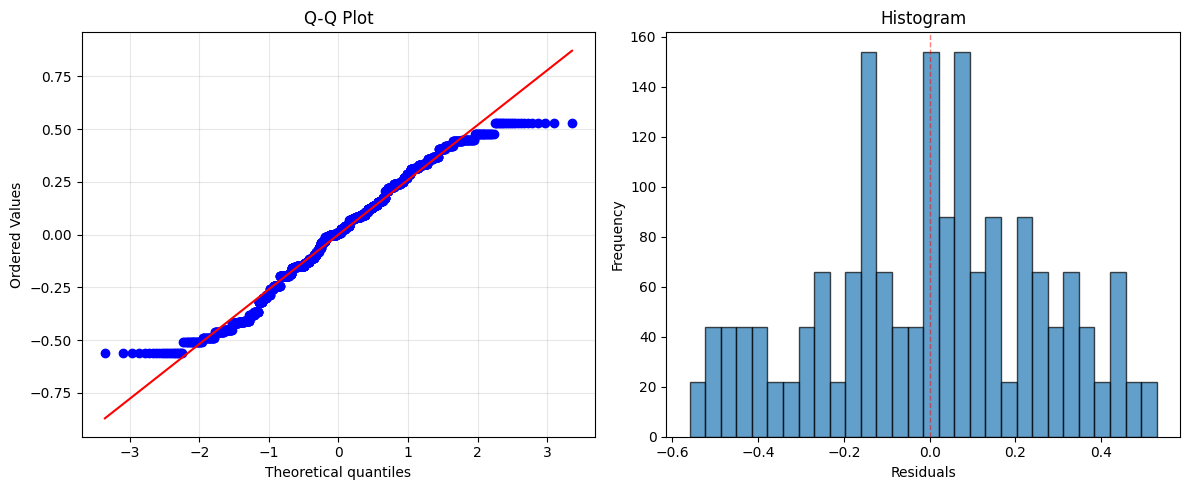
\includegraphics[width=\textwidth]{qq2.png}
    \end{minipage}
    \caption{Between-country residuals}
    \label{fig:residuals}
    \end{figure} 

The plots on the left of Figure \ref{fig:residuals} are  Q-Q plots, they show quantile-quantile comparisons and align pretty well with line with the 45 degree slope thereby demonstrating theoretical normal distribution; the histograms on the right display empirical normal distributions.

\section{Interpretation of Within vs. Between Effects}

The larger within-country effect for low-income countries compared to the between-country effect requires explanation. Between-country effects reflect structural, long-run differences—they compare countries' average GDP and mortality over the entire 22-year period. Within-country effects capture year-to-year GDP growth and its immediate impact on mortality. Because within-country variation is more volatile (annual changes rather than averages), the coefficient magnitude is larger, yielding more prominent mortality reductions for the same percentage GDP increase.


\end{document}